\chapter{Tabel Periodik: Pandangan Pertama}\label{ch:g9:periodic-table-first-look}

Di dinding hampir setiap ruang kelas kimia tergantung bagan yang sama:
118 kotak, masing-masing berisi lambang dan angka, tersusun dalam baris
dan kolom dengan bentuk yang aneh --- menara tinggi di kedua sisinya,
lekukan di tengah, dan dua baris lepas di bawahnya. Ketika pertama kali
digambar, pada tahun 1869, bagan itu memuat sekitar enam puluh kotak dan
beberapa kotak kosong. Penyusunnya cukup berani menguraikan unsur-unsur
yang suatu hari akan mengisi celah-celah itu --- dan ia benar.

\begin{recall}
\omterm{def:g9:inside-the-atom:element}{Unsur kimia} adalah himpunan \omterm{def:g7:atoms-and-molecules:atom}{atom} dengan \omterm{def:g9:inside-the-atom:atomic-number}{nomor atom} $Z$ yang sama, yaitu
banyaknya \omterm{def:g9:inside-the-atom:proton}{proton} di dalam inti (\cref{ch:g9:inside-the-atom}). Setiap
unsur memiliki lambang, satu huruf kapital yang kadang diikuti satu
huruf kecil (\cref{ch:g7:atoms-and-molecules}). \omterm{def:g9:periodic-table-first-look:metal}{Logam} seperti besi,
seng, dan aluminium membentuk \omterm{def:g9:ions:ion}{ion} positif (\cref{ch:g9:ions}).
\end{recall}

\section{Sebuah tabel unsur-unsur}

\begin{definition}[Tabel periodik]\label{def:g9:periodic-table-first-look:periodic-table}
Yang disebut \emph{tabel periodik}\index{tabel periodik} adalah daftar
semua \omterm{def:g9:inside-the-atom:element}{unsur kimia} menurut \omterm{def:g9:inside-the-atom:atomic-number}{nomor atom} yang makin besar, $Z = 1$ sampai
$Z = 118$, yang disusun dalam baris-baris sedemikian rupa sehingga
unsur-unsur yang sifatnya mirip berada dalam kolom yang sama.
\end{definition}

\begin{definition}[Periode dan golongan]\label{def:g9:periodic-table-first-look:period}
Sebuah baris \omterm{def:g9:periodic-table-first-look:periodic-table}{tabel periodik} disebut \emph{periode}\index{periode}; ada
tujuh periode. Sebuah kolom disebut \emph{golongan}\index{golongan}; ada
delapan belas golongan, diberi nomor 1 sampai 18 dari kiri ke kanan.
Kedua baris yang dicetak di bawah tabel sebenarnya termasuk periode 6
dan 7; keduanya dipisahkan hanya agar tabelnya tidak terlalu lebar.
\end{definition}

\begin{omfigure}
\omperiodictable[colour=metals, legend=true, cell=0.86cm]

{\small \omterm{def:g9:periodic-table-first-look:periodic-table}{Tabel periodik}. Setiap kotak memuat \omterm{def:g9:inside-the-atom:atomic-number}{nomor atom} dan lambang.
Warna: \omterm{def:g9:periodic-table-first-look:metal}{logam}, metaloid (unsur di antara \omterm{def:g9:periodic-table-first-look:metal}{logam} dan \omterm{def:g9:periodic-table-first-look:metal}{nonlogam}), dan
\omterm{def:g9:periodic-table-first-look:metal}{nonlogam}, menurut penggolongan yang lazim.}
\end{omfigure}

\begin{method}[Membaca tabel periodik]\label{met:g9:periodic-table-first-look:read}
Untuk menempatkan sebuah unsur:
\begin{enumerate}
  \item carilah kotaknya dari lambang atau \omterm{def:g9:inside-the-atom:atomic-number}{nomor atomnya};
  \item barisnya menunjukkan \omterm{def:g9:periodic-table-first-look:period}{periodenya}, kolomnya menunjukkan \omterm{def:g9:periodic-table-first-look:period}{golongannya};
  \item warnanya menyatakan apakah unsur itu \omterm{def:g9:periodic-table-first-look:metal}{logam} atau \omterm{def:g9:periodic-table-first-look:metal}{nonlogam}.
\end{enumerate}
Natrium, \ce{Na}, $Z = 11$: \omterm{def:g9:periodic-table-first-look:period}{periode} 3, \omterm{def:g9:periodic-table-first-look:period}{golongan} 1, sebuah \omterm{def:g9:periodic-table-first-look:metal}{logam}. Klorin,
\ce{Cl}, $Z = 17$: \omterm{def:g9:periodic-table-first-look:period}{periode} 3, \omterm{def:g9:periodic-table-first-look:period}{golongan} 17, sebuah \omterm{def:g9:periodic-table-first-look:metal}{nonlogam}.
\end{method}

\section{Logam dan nonlogam}

\begin{definition}[Logam dan nonlogam]\label{def:g9:periodic-table-first-look:metal}
Sebuah \emph{logam}\index{logam} adalah unsur yang, sebagai \omterm{def:g6:pure-substances-and-mixtures:pure-substance}{zat murni},
mengilap ketika baru dipotong, menghantarkan listrik dan panas dengan
baik, dapat dibengkokkan atau ditempa, dan membentuk \omterm{def:g9:ions:ion}{ion} positif. Sebuah
\emph{nonlogam}\index{nonlogam} tidak memiliki sifat-sifat itu: banyak
nonlogam berupa gas (oksigen, nitrogen, klorin), nonlogam yang padat
kusam dan rapuh (belerang, karbon sebagai batu bara), dan nonlogam
cenderung membentuk \omterm{def:g9:ions:ion}{ion} negatif atau berbagi \omterm{def:g9:inside-the-atom:nucleus}{elektron} dalam \omterm{def:g7:atoms-and-molecules:molecule}{molekul}.
\end{definition}

\begin{proposition}[Letak keduanya]\label{prop:g9:periodic-table-first-look:where}
Sekitar empat dari lima unsur adalah \omterm{def:g9:periodic-table-first-look:metal}{logam}; \omterm{def:g9:periodic-table-first-look:metal}{logam} mengisi bagian kiri
dan tengah tabel. \omterm{def:g9:periodic-table-first-look:metal}{Nonlogam} berada di kanan atas, dengan hidrogen sendirian
di kiri atas. Di sepanjang perbatasan di antara keduanya, beberapa unsur
--- boron, silikon, germanium, arsen, antimon, telurium --- memiliki
sifat di antara keduanya: metaloid.
\end{proposition}

\section{Kolom-kolom yang berperilaku sama}

\begin{proposition}[Unsur-unsur segolongan berperilaku sama]\label{prop:g9:periodic-table-first-look:alike}
Unsur-unsur dalam satu \omterm{def:g9:periodic-table-first-look:period}{golongan} bereaksi dengan cara yang mirip dan
membentuk senyawa yang mirip. Litium, natrium, dan kalium, di bagian
atas \omterm{def:g9:periodic-table-first-look:period}{golongan} 1, adalah \omterm{def:g9:periodic-table-first-look:metal}{logam} lunak yang bereaksi dengan air sambil
melepaskan hidrogen; reaksinya makin hebat ke arah bawah \omterm{def:g9:periodic-table-first-look:period}{golongan}.
Fluorin, klorin, bromin, dan iodin, di \omterm{def:g9:periodic-table-first-look:period}{golongan} 17, adalah \omterm{def:g9:periodic-table-first-look:metal}{nonlogam}
berwarna yang bereaksi dengan \omterm{def:g9:periodic-table-first-look:metal}{logam} membentuk garam. Helium, neon, argon,
dan unsur-unsur lain \omterm{def:g9:periodic-table-first-look:period}{golongan} 18 hampir tidak bereaksi dengan apa pun.
\end{proposition}

\begin{inthelab}[Litium, natrium, dan kalium dalam air]
Di balik layar pelindung, guru menjatuhkan sepotong litium sebesar
sebutir beras ke dalam baskom besar berisi air: litium itu berdesis
pelan. Sepotong natrium seukuran itu berlari-lari di permukaan air,
meleleh menjadi bola keperakan. Kalium langsung menyala dengan api
berwarna ungu muda. Ketiganya melepaskan hidrogen dan meninggalkan
\omterm{def:g9:acids-bases-ph:acidic}{larutan basa}.
\end{inthelab}

\begin{safety}{\ghs[0.82cm]{GHS02}\ghs[0.82cm]{GHS05}}
% ledger: ghs:Na
Natrium: jika bersentuhan dengan air melepaskan gas mudah menyala yang
dapat menyala sendiri (GHS02); menyebabkan luka bakar parah (GHS05).
Natrium disimpan di dalam minyak dan hanya ditangani oleh guru, dengan
penjepit, dalam potongan-potongan kecil.
\end{safety}

\section{Gagasan Mendeleev}

\begin{history}[Celah-celah Mendeleev, 1869--1886]
Pada tahun 1869 Dmitri Mendeleev menyusun unsur-unsur yang dikenal pada
masa itu menurut massa \omterm{def:g7:atoms-and-molecules:atom}{atom} relatif yang makin besar --- massa \omterm{def:g7:atoms-and-molecules:atom}{atom-atomnya}
dibandingkan dengan massa \omterm{def:g7:atoms-and-molecules:atom}{atom} hidrogen --- dan menempatkan unsur-unsur
yang sifatnya mirip berdampingan. Di tempat pola itu menuntutnya, ia
membiarkan celah untuk unsur-unsur yang belum ditemukan siapa pun, dan
pada tahun 1871 ia menguraikan sifat-sifatnya: di bawah silikon, sebuah
``eka-silikon'' yang massa \omterm{def:g7:atoms-and-molecules:atom}{atom} relatifnya akan sekitar 72. Pada tahun 1886 ahli
kimia Clemens Winkler menemukan germanium dalam \omterm{def:g5:raw-materials-and-recycling:raw-material}{bijih} perak, mengukur
massa \omterm{def:g7:atoms-and-molecules:atom}{atom} relatifnya sebesar 72.3, dan mendapati bahwa unsur itulah yang hilang.
Galium (1875) dan skandium (1879) juga mengisi celah-celah yang
ditinggalkan Mendeleev.
\end{history}

\begin{omfigure}
\begin{minipage}[b]{0.32\linewidth}\centering
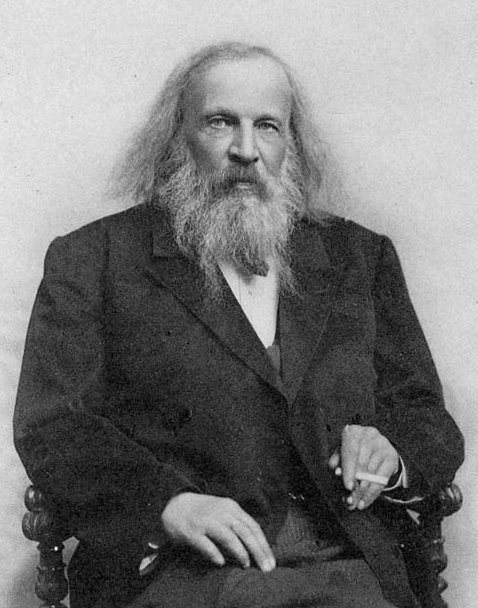
\includegraphics[width=\linewidth]{images/book1/mendeleev.jpg}

{\small Dmitri Mendeleev (1834--1907).}
\end{minipage}\hfill
\begin{minipage}[b]{0.6\linewidth}\centering
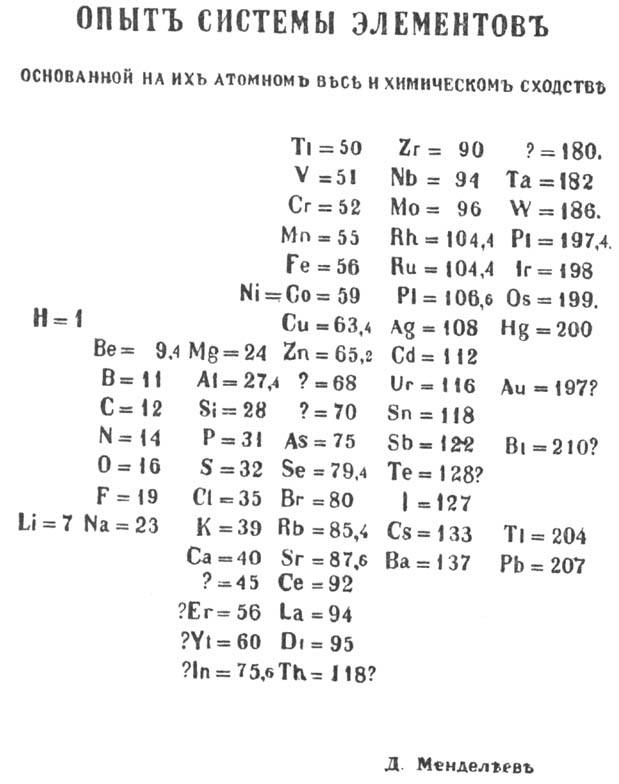
\includegraphics[width=0.85\linewidth]{images/book1/mendeleev-1869.jpg}

{\small Tabel Mendeleev tahun 1869, dalam bahasa Rusia. Di samping
Si $= 28$ dan Al $= 27.4$, celah ``? $= 70$'' dan ``? $= 68$'' menanti
germanium dan galium.}
\end{minipage}
\end{omfigure}

\begin{remark}[Urutan menurut nomor atom]\label{rem:g9:periodic-table-first-look:order}
Mendeleev mengurutkan unsur-unsur menurut massa \omterm{def:g7:atoms-and-molecules:atom}{atom} relatif, dan harus
menukar beberapa pasang, seperti telurium dan iodin, agar keluarga-keluarga
unsur tetap bersatu. Sekarang tabel itu diurutkan menurut \omterm{def:g9:inside-the-atom:atomic-number}{nomor atom},
yang ditemukan kemudian, dan pertukaran itu tidak diperlukan lagi.
\end{remark}

\section{Latihan}

\begin{exercise}[$\star$]\label{exo:g9:periodic-table-first-look:1}
Menurut urutan apa unsur-unsur ditempatkan dalam \omterm{def:g9:periodic-table-first-look:periodic-table}{tabel periodik}?
\end{exercise}

\begin{exercise}[$\star$]\label{exo:g9:periodic-table-first-look:2}
Tentukan \omterm{def:g9:periodic-table-first-look:period}{periode} dan \omterm{def:g9:periodic-table-first-look:period}{golongan} dari: karbon ($Z = 6$), magnesium
($Z = 12$), argon ($Z = 18$).
\end{exercise}

\begin{exercise}[$\star$]\label{exo:g9:periodic-table-first-look:3}
\omterm{def:g9:periodic-table-first-look:metal}{Logam} atau \omterm{def:g9:periodic-table-first-look:metal}{nonlogam}: besi, belerang, tembaga, oksigen, aluminium, klorin?
\end{exercise}

\begin{exercise}[$\star$]\label{exo:g9:periodic-table-first-look:4}
Unsur apa yang tepat berada di bawah natrium dalam tabel? Tepat di bawah
klorin?
\end{exercise}

\begin{exercise}[$\star\star$]\label{exo:g9:periodic-table-first-look:5}
Dengan tabel itu, sebutkan unsur pada \omterm{def:g9:periodic-table-first-look:period}{periode} 4 dan \omterm{def:g9:periodic-table-first-look:period}{golongan} 2, serta
unsur pada \omterm{def:g9:periodic-table-first-look:period}{periode} 2 dan \omterm{def:g9:periodic-table-first-look:period}{golongan} 15.
\end{exercise}

\begin{exercise}[$\star\star$]\label{exo:g9:periodic-table-first-look:6}
Mengapa kalium dapat diharapkan bereaksi dengan air, seperti natrium?
\end{exercise}

\begin{exercise}[$\star\star$]\label{exo:g9:periodic-table-first-look:7}
Sebuah unsur yang mengilap menghantarkan listrik dan membentuk \omterm{def:g9:ions:ion}{ion}
\ce{X^{2+}}. Apakah unsur itu \omterm{def:g9:periodic-table-first-look:metal}{logam} atau \omterm{def:g9:periodic-table-first-look:metal}{nonlogam}? Jelaskan.
\end{exercise}

\begin{exercise}[$\star\star$]\label{exo:g9:periodic-table-first-look:8}
Mengapa Mendeleev membiarkan celah-celah dalam tabelnya? Mengapa hal ini
menjadi kekuatan tabelnya dan bukan kelemahannya?
\end{exercise}

\begin{exercise}[$\star\star$]\label{exo:g9:periodic-table-first-look:9}
Lihatlah tabel Mendeleev tahun 1869. Massa \omterm{def:g7:atoms-and-molecules:atom}{atom} relatif berapa yang
diberikannya untuk karbon dan untuk oksigen? Dua celah mana, yang
ditandai tanda tanya, muncul di samping aluminium dan silikon?
\end{exercise}

\begin{exercise}[$\star\star$]\label{exo:g9:periodic-table-first-look:10}
Berapa unsur yang ada dalam \omterm{def:g9:periodic-table-first-look:period}{periode} 2? Dalam \omterm{def:g9:periodic-table-first-look:period}{periode} 4?
\end{exercise}

\begin{exercise}[$\star\star\star$]\label{exo:g9:periodic-table-first-look:11}
Helium, neon, dan argon hampir tidak bereaksi dengan apa pun. Di
\omterm{def:g9:periodic-table-first-look:period}{golongan} mana unsur-unsur itu berada? Untuk apa unsur-unsur itu dapat
dipakai, mengingat sifat ini?
\end{exercise}

\begin{exercise}[$\star\star\star$]\label{exo:g9:periodic-table-first-look:12}
Galium, di bawah aluminium, ditemukan pada tahun 1875. Mendeleev telah
meramalkan untuknya massa \omterm{def:g7:atoms-and-molecules:atom}{atom} relatif yang mendekati rata-rata kedua
tetangganya, aluminium (27.0) dan indium (114.8). Hitung rata-rata itu.
(Galium: 69.7.)
\end{exercise}

\section{Soal: Celah Mendeleev}

\begin{problem}[{Soal akhir pekan --- meramalkan massa atom relatif sebuah unsur
yang hilang dari keempat tetangganya}]
\label{pb:g9:periodic-table-first-look:1}
% ledger: aw:Si, aw:Sn, aw:Ga, aw:As, aw:Ge, mend:eka-si-aw, ge:winkler-aw
Pada tahun 1871 Mendeleev meramalkan sifat-sifat eka-silikon, unsur yang
hilang di bawah silikon. Salah satu gagasannya adalah bahwa sifat sebuah
unsur terletak di antara sifat-sifat tetangganya di atas dan di bawah,
di kiri dan di kanan. Massa \omterm{def:g7:atoms-and-molecules:atom}{atom} relatif keempat tetangga celah itu menurut
nilai sekarang adalah: silikon 28.1 (di atas), timah 118.7 (di bawah),
galium 69.7 (di kiri), arsen 74.9 (di kanan).

\medskip
\noindent\textbf{Bagian I --- Celahnya.}
\begin{enumerate}
  \item Dengan \omterm{def:g9:periodic-table-first-look:periodic-table}{tabel periodik} dalam bab ini, tentukan \omterm{def:g9:inside-the-atom:atomic-number}{nomor atom}, \omterm{def:g9:periodic-table-first-look:period}{periode},
        dan \omterm{def:g9:periodic-table-first-look:period}{golongan} germanium, unsur yang mengisi celah itu.
  \item Unsur apa yang berada di atasnya, di bawahnya, di kirinya, dan di
        kanannya?
  \item Apakah germanium \omterm{def:g9:periodic-table-first-look:metal}{logam}, \omterm{def:g9:periodic-table-first-look:metal}{nonlogam}, atau metaloid?
  \item Mengapa Mendeleev menduga bahwa unsur yang hilang itu mirip
        dengan silikon?
\end{enumerate}

\medskip
\noindent\textbf{Bagian II --- Rata-rata.}
\begin{enumerate}[resume]
  \item Hitung rata-rata massa \omterm{def:g7:atoms-and-molecules:atom}{atom} relatif unsur-unsur di atas dan di bawah
        celah itu.
  \item Hitung rata-rata massa \omterm{def:g7:atoms-and-molecules:atom}{atom} relatif unsur-unsur di kiri dan di kanan.
  \item Manakah di antara kedua rata-rata itu yang lebih dekat dengan
        massa \omterm{def:g7:atoms-and-molecules:atom}{atom} relatif germanium yang sebenarnya, 72.6? Mengapa demikian?
  \item Dalam tabelnya tahun 1869, Mendeleev menulis ``? $= 70$'' untuk
        celah ini. Berapa selisih perkiraannya?
\end{enumerate}

\medskip
\noindent\textbf{Bagian III --- Ramalannya.}
\begin{enumerate}[resume]
  \item Hitung rata-rata keempat tetangga itu, sampai satu angka di
        belakang koma.
  \item Pada tahun 1871 Mendeleev meramalkan 72; pada tahun 1886 Winkler
        mengukur 72.3. Bandingkan dengan rata-ratamu.
  \item Mengapa penemuan germanium meyakinkan banyak ahli kimia bahwa
        tabel Mendeleev benar?
  \item Nyatakan ramalanmu: massa \omterm{def:g7:atoms-and-molecules:atom}{atom} relatif eka-silikon dari rata-rata keempat
        tetangganya.
\end{enumerate}
\end{problem}
